\appendix
\chapter{Appendix}  \label{chap:A}

\begin{figure}
    \begin{adjustbox}{minipage=\dimexpr\textwidth-2\fboxsep-2\fboxrule,fbox}
        \begin{subfigure}[b]{0.475\textwidth}
            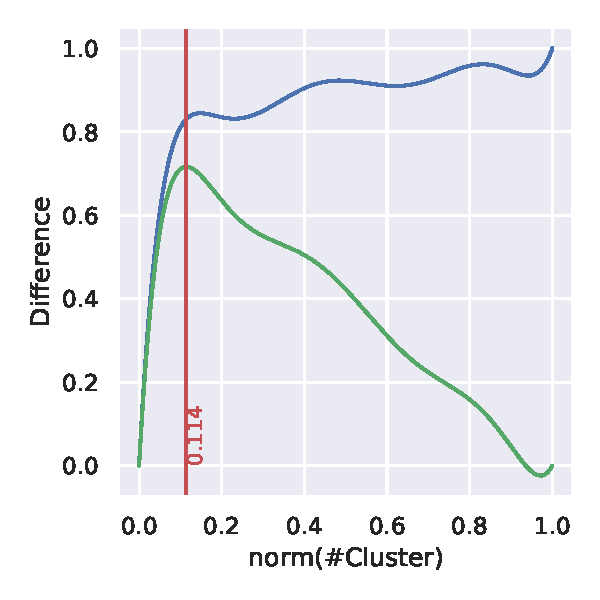
\includegraphics[width=\textwidth]{PCA/Cluster_Knee_Segment_6.pdf}
            \caption[Kneedle Algorithm]{\textbf{Kneedle Algorithm}}
            \label{fig:A.0.1a}
        \end{subfigure}
        \hfill
        \begin{subfigure}[b]{0.475\textwidth}
            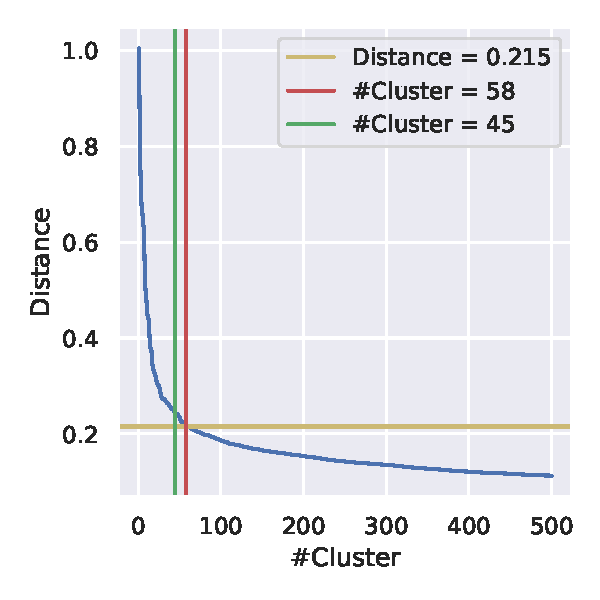
\includegraphics[width=\textwidth]{PCA/Cluster_Elbow_Knee_Segment_6.pdf}
            \caption[Kneedle Knee]{\textbf{Kneedle Knee}}
            \label{fig:A.0.1b}
        \end{subfigure}
        \vskip\baselineskip
        \begin{subfigure}[b]{0.475\textwidth}
            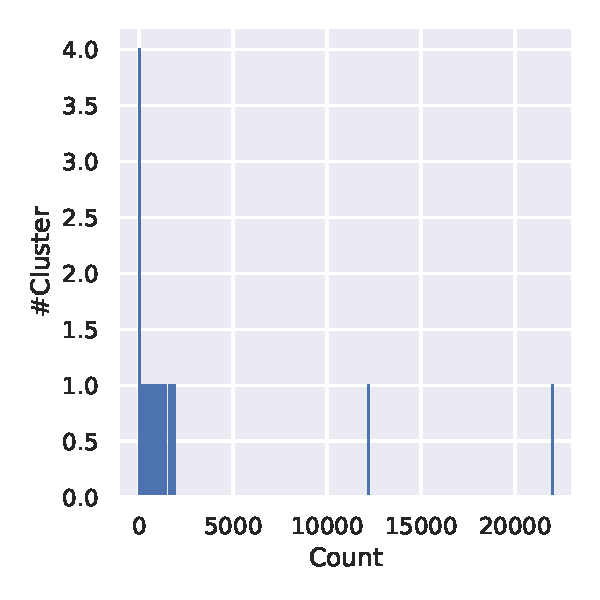
\includegraphics[width=\textwidth]{PCA/Cluster_Distribution_Segment_6.pdf}
            \caption[Cluster Distribution]{\textbf{Cluster Distribution}}
            \label{fig:A.0.1c}
        \end{subfigure}
        \hfill
        \begin{subfigure}[b]{0.475\textwidth}
            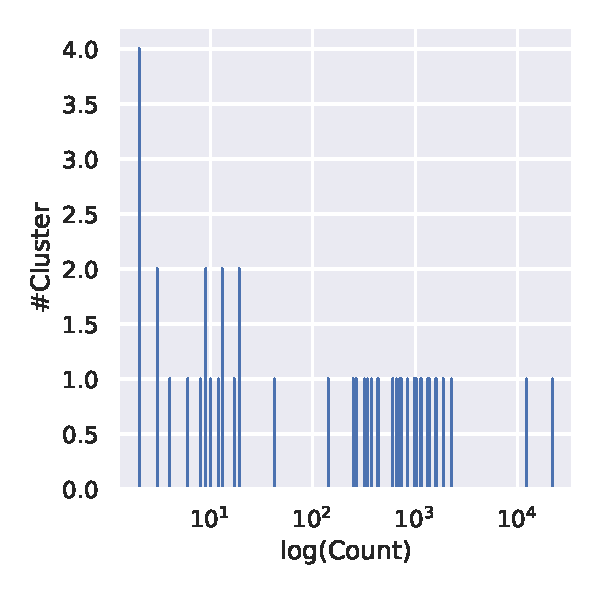
\includegraphics[width=\textwidth]{PCA/Cluster_Distribution_Log_Segment_6.pdf}
            \caption[Logarithmic Distribution]{\textbf{Logarithmic Distribution}}
            \label{fig:A.0.1d}
        \end{subfigure}
    \end{adjustbox}
    \caption[Knee based Segment 6 Clustering with PCA]{\textbf{Knee based Segment 6 Clustering with PCA.}.}
    \label{fig:A.0.1}
\end{figure}

\begin{figure}
    \begin{adjustbox}{minipage=\dimexpr\textwidth-2\fboxsep-2\fboxrule,fbox}
        \begin{subfigure}[b]{0.475\textwidth}
            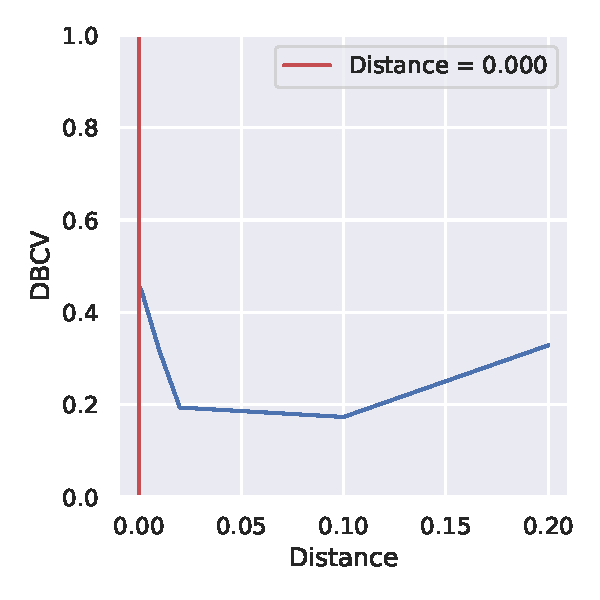
\includegraphics[width=\textwidth]{PCA/Cluster_DBCV_Segment_6.pdf}
            \caption[Cosine]{\textbf{DBCV Exploration}}
            \label{fig:A.0.2a}
        \end{subfigure}
        \hfill
        \begin{subfigure}[b]{0.475\textwidth}
            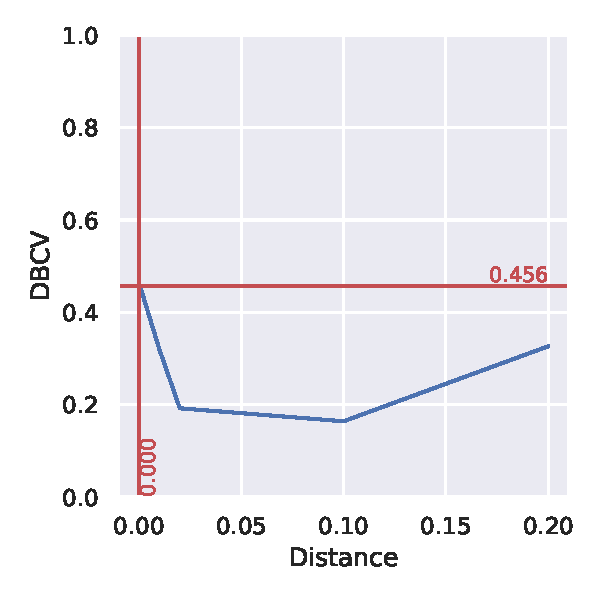
\includegraphics[width=\textwidth]{PCA/Cluster_Elbow_DBCV_Segment_6.pdf}
            \caption[DBCV Knee]{\textbf{DBCV Knee}}
            \label{fig:A.0.2b}
        \end{subfigure}
        \vskip\baselineskip
        \begin{subfigure}[b]{0.475\textwidth}
            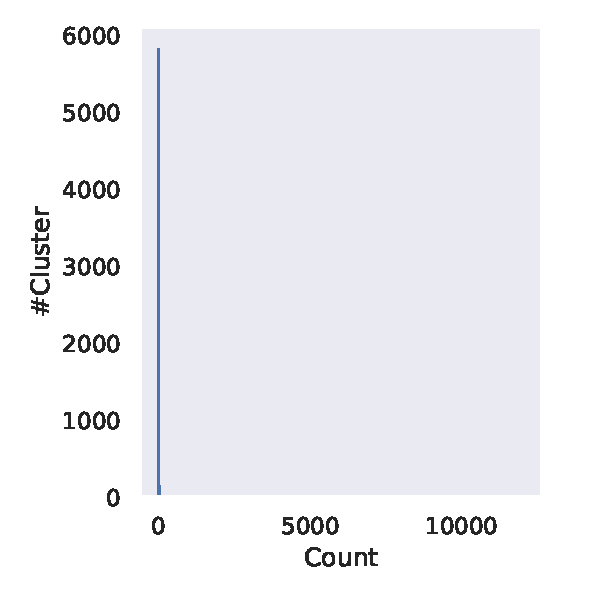
\includegraphics[width=\textwidth]{PCA/Cluster_Distribution_Segment_6_alternative.pdf}
            \caption[Cluster Distribution]{\textbf{Cluster Distribution}}
            \label{fig:A.0.2c}
        \end{subfigure}
        \hfill
        \begin{subfigure}[b]{0.475\textwidth}
            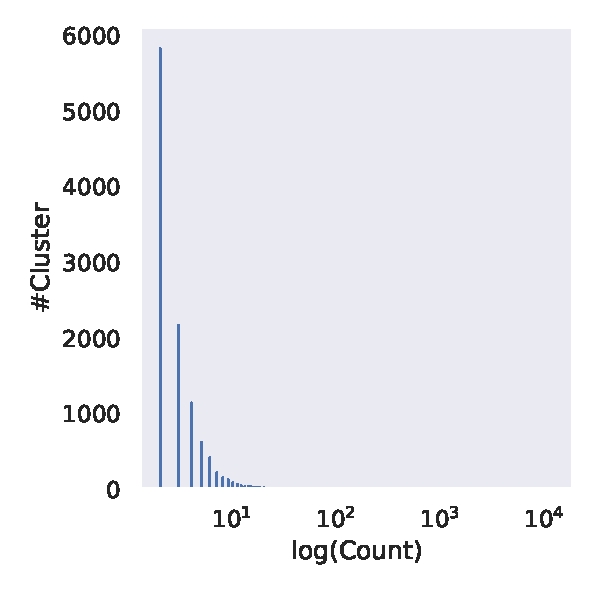
\includegraphics[width=\textwidth]{PCA/Cluster_Distribution_Log_Segment_6_alternative.pdf}
            \caption[Logarithmic Distribution]{\textbf{Logarithmic Distribution}}
            \label{fig:A.0.2d}
        \end{subfigure}
    \end{adjustbox}
    \caption[DBCV based Segment 6 Clustering with PCA]{\textbf{DBCV based Segment 6 Clustering with PCA.}.}
    \label{fig:A.0.2}
\end{figure}

\begin{figure}
    \begin{adjustbox}{minipage=\dimexpr\textwidth-2\fboxsep-2\fboxrule,fbox}
        \begin{subfigure}[b]{0.475\textwidth}
            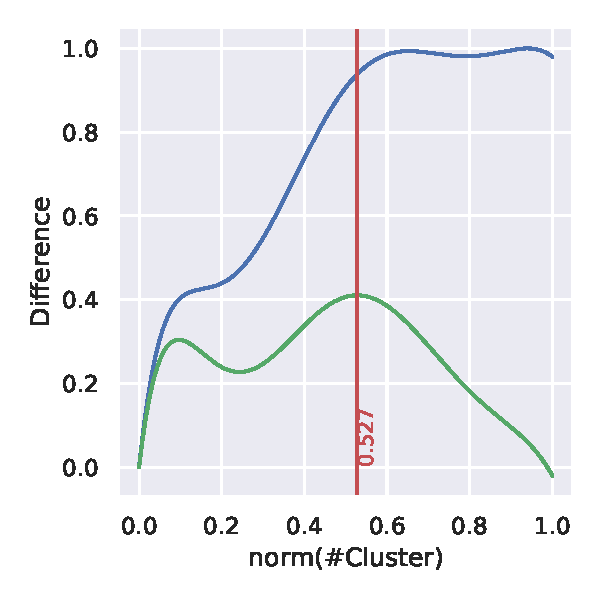
\includegraphics[width=\textwidth]{UMAP/Cluster_Knee_Segment_6.pdf}
            \caption[Kneedle Algorithm]{\textbf{Kneedle Algorithm}}
            \label{fig:A.0.3a}
        \end{subfigure}
        \hfill
        \begin{subfigure}[b]{0.475\textwidth}
            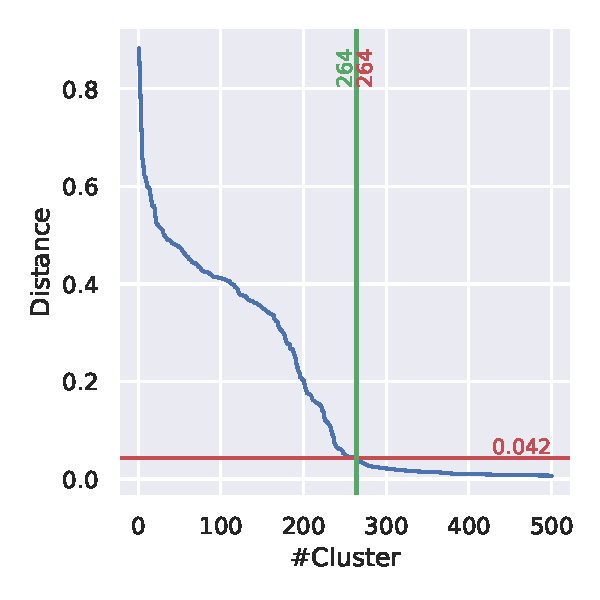
\includegraphics[width=\textwidth]{UMAP/Cluster_Elbow_Knee_Segment_6.pdf}
            \caption[Kneedle Knee]{\textbf{Kneedle Knee}}
            \label{fig:A.0.3b}
        \end{subfigure}
        \vskip\baselineskip
        \begin{subfigure}[b]{0.475\textwidth}
            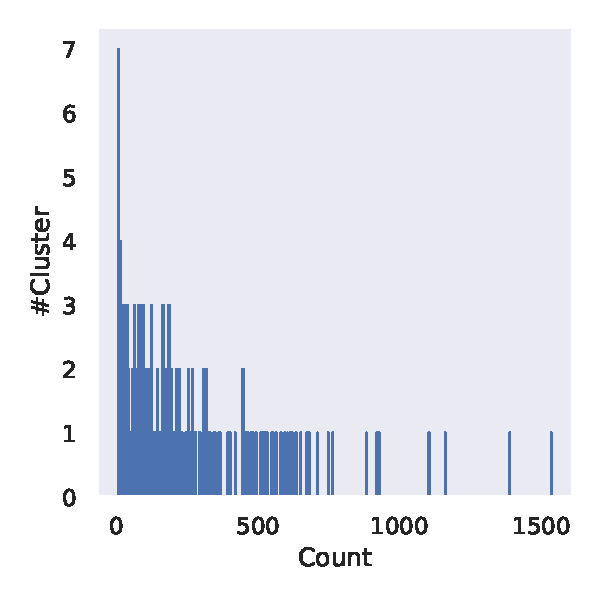
\includegraphics[width=\textwidth]{UMAP/Cluster_Distribution_Segment_6.pdf}
            \caption[Cluster Distribution]{\textbf{Cluster Distribution}}
            \label{fig:A.0.3c}
        \end{subfigure}
        \hfill
        \begin{subfigure}[b]{0.475\textwidth}
            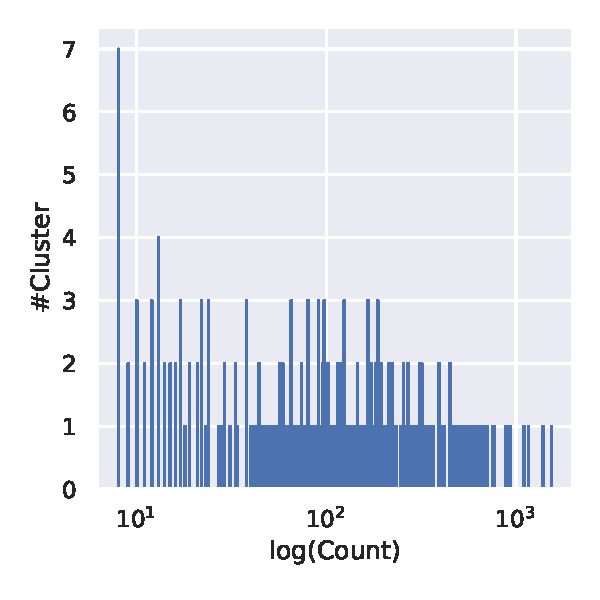
\includegraphics[width=\textwidth]{UMAP/Cluster_Distribution_Log_Segment_6.pdf}
            \caption[Logarithmic Distribution]{\textbf{Logarithmic Distribution}}
            \label{fig:A.0.3d}
        \end{subfigure}
    \end{adjustbox}
    \caption[Knee based Segment 6 Clustering with UMAP]{\textbf{Knee based Segment 6 Clustering with UMAP.}.}
    \label{fig:A.0.3}
\end{figure}

\begin{figure}
    \begin{adjustbox}{minipage=\dimexpr\textwidth-2\fboxsep-2\fboxrule,fbox}
        \begin{subfigure}[b]{0.475\textwidth}
            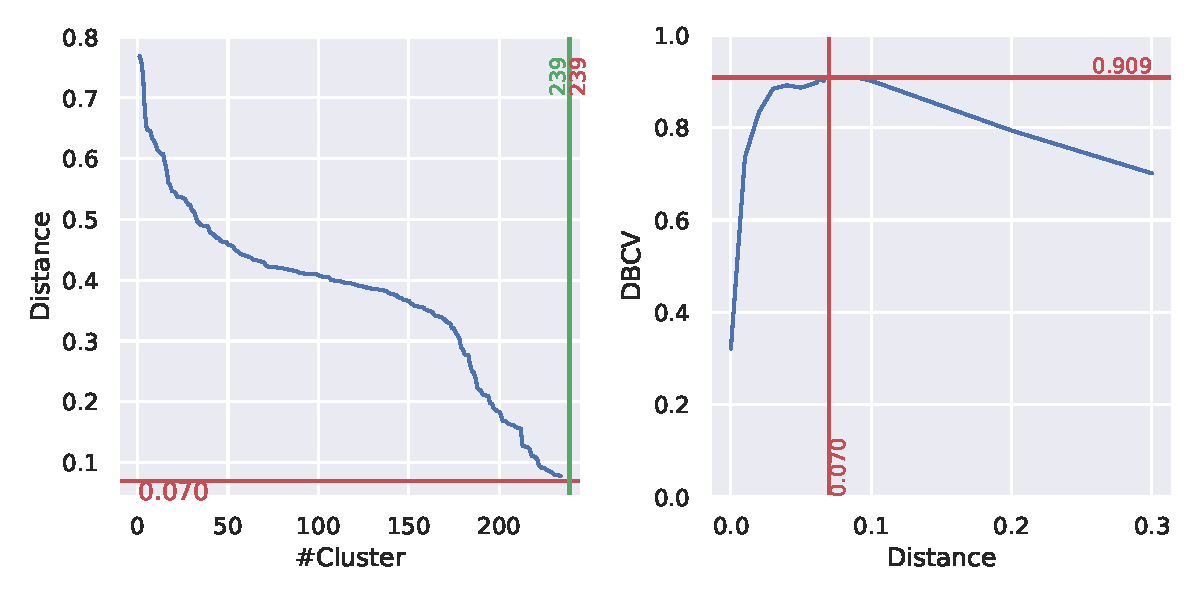
\includegraphics[width=\textwidth]{UMAP/Cluster_DBCV_Segment_6.pdf}
            \caption[Cosine]{\textbf{DBCV Exploration}}
            \label{fig:A.0.4a}
        \end{subfigure}
        \hfill
        \begin{subfigure}[b]{0.475\textwidth}
            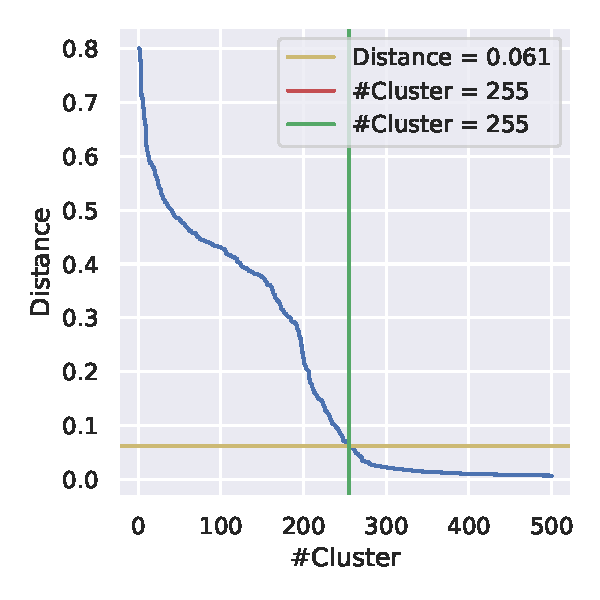
\includegraphics[width=\textwidth]{UMAP/Cluster_Elbow_DBCV_Segment_6.pdf}
            \caption[DBCV Knee]{\textbf{DBCV Knee}}
            \label{fig:A.0.4b}
        \end{subfigure}
        \vskip\baselineskip
        \begin{subfigure}[b]{0.475\textwidth}
            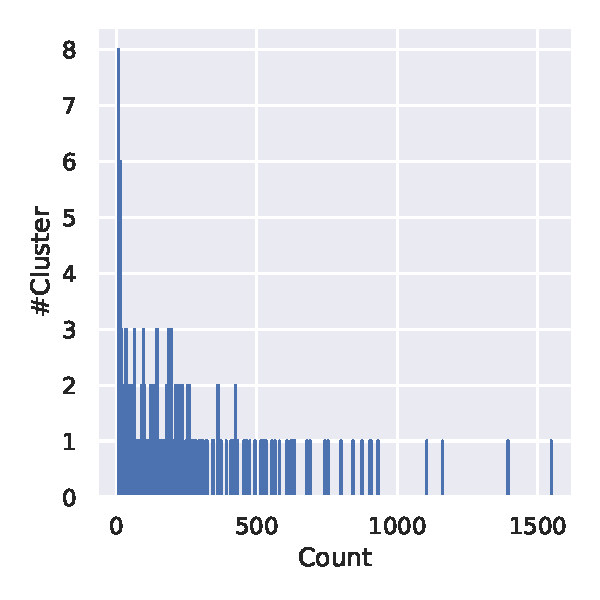
\includegraphics[width=\textwidth]{UMAP/Cluster_Distribution_Segment_6_alternative.pdf}
            \caption[Cluster Distribution]{\textbf{Cluster Distribution}}
            \label{fig:A.0.4c}
        \end{subfigure}
        \hfill
        \begin{subfigure}[b]{0.475\textwidth}
            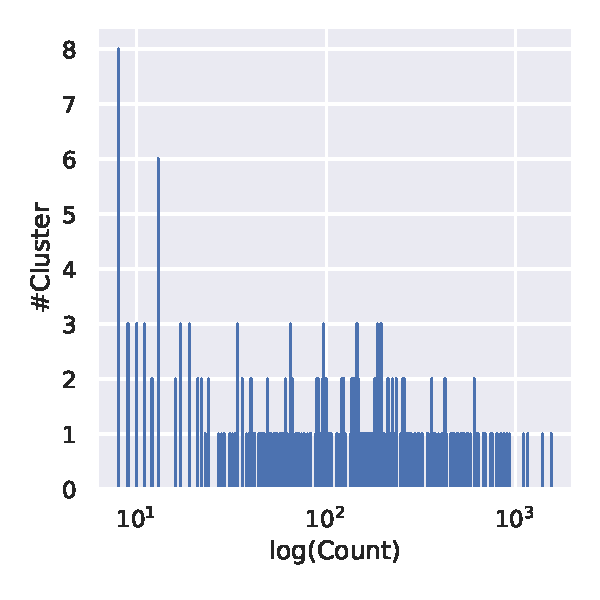
\includegraphics[width=\textwidth]{UMAP/Cluster_Distribution_Log_Segment_6_alternative.pdf}
            \caption[Logarithmic Distribution]{\textbf{Logarithmic Distribution}}
            \label{fig:A.0.4d}
        \end{subfigure}
    \end{adjustbox}
    \caption[DBCV based Segment 6 Clustering with UMAP]{\textbf{DBCV based Segment 6 Clustering with UMAP.}.}
    \label{fig:A.0.4}
\end{figure}

\begin{table}[!hbt]
    \caption[Cluster Database with PCA]{\textbf{Cluster Database with PCA.}.}
    \label{tab:A.0.5}
    \pgfplotstabletypeset[
        every head row/.style={
            before row={
                \toprule
            },
            after row={
                \midrule
            },
        },
        every last row/.style={
            after row={
                ... & ... & ... & ... & ... & ... & ... \\
                \bottomrule
            },
        },
        begin table=\begin{tabular*}{\textwidth},
        end table=\end{tabular*},
        columns={0,1,2,3,4,5,6},
        columns/0/.style={string type,multicolumn names=l,column name=\textbf{Accession}, column type=@{\extracolsep{\fill} }r},
        columns/1/.style={multicolumn names=l,column name=\textbf{Segment}, column type=r},
        columns/2/.style={multicolumn names=l,column name=\textbf{Cluster}, column type=r},
        columns/3/.style={string type,multicolumn names=l,column name=\textbf{H}, column type=r},
        columns/4/.style={string type,multicolumn names=l,column name=\textbf{Centroid}, column type=r},
        columns/5/.style={string type,multicolumn names=l,column name=\textbf{N}, column type=r},
        columns/6/.style={string type,multicolumn names=l,column name=\textbf{Strain}, column type=r},
    ]
    {PCA/cluster_head.csv}
\end{table}